%!TEX TS-program = xelatex
%!TEX encoding = UTF-8 Unicode
 
\documentclass[11pt]{extarticle}
% extarticle is like article but can handle 8pt, 9pt, 10pt, 11pt, 12pt, 14pt, 17pt, and 20pt text

\def \ititle {Which Joint Actions Ground Social Cognition}
\def \isubtitle {}
\def \iauthor {Stephen A. Butterfill}
\def \iemail{s.butterfill@warwick.ac.uk}
\date{}

%for strikethrough
\usepackage[normalem]{ulem}

\input{$HOME/Documents/submissions/preamble_steve_handout}

\bibpunct{}{}{,}{s}{}{,}  %use superscript TICS style bib
%remove hanging indent for TICS style bib
%TODO doesnt work
\setlength{\bibhang}{0em}
%\setlength{\bibsep}{0.5em}


%itemize bullet should be dash
\renewcommand{\labelitemi}{$-$}

\begin{document}

\begin{multicols}{3}

\setlength\footnotesep{1em}


\bibliographystyle{newapa} %apalike

%\maketitle
%\tableofcontents



\

\begin{center}
{\Large
\textbf{What is Joint Action?}
}

%JAM4, Vienna, July 2011
%Stephen A. Butterfill
<s.butterfill@warwick.ac.uk>

\end{center}




\section{History}

\emph{Ask a psychologist}
`joint action [is] any form of social interaction whereby two or more individuals coordinate their actions in space and time to bring about a change in the environment.'%
\citep{Sebanz:2006yq}

\emph{Ask a philosopher} 
`I take a collective action to involve a collective intention.'  \citep%[p.\ 5]
{Gilbert:2006wr}
%
`The sine qua non of collaborative action is a joint goal [shared intention] and a joint commitment.' 
\citep%[p.\ 181]
{tomasello:2008origins}
%
`The key property of joint action lies in its internal component \ldots \ in the participants’ having a ``collective'' or ``shared'' intention.' \citep%[pp. 444-5]
{alonso_shared_2009}
%
`Shared intentionality is the foundation upon which joint action is built.' \citep%[p.\ 381]
{Carpenter:2009wq}
%
`It is precisely the meshing and sharing of psychological states \ldots \ that holds the key to understanding how humans have achieved their sophisticated and numerous forms of joint activity.'
\citep%[p.\ 369]
{Call:2009fk}


\section{The Challenge}

Show that a notion of joint action is already contained in a notion of action.

\section{The Constraint}

Any notion of joint action is 
\begin{itemize}
\item central to a tangle of philosophical and scientific questions  commonly taken to be questions about joint action, and
\item such that an implicit conception of it is available through reflection on many or all of the cases commonly taken to be paradigmatic.
\end{itemize}


\section{Towards a Solution}


\subsection{First attempt} 
A joint action is an action with two or more agents\citep{ludwig_collective_2007}

\emph{Objection} 
`our primitive actions, the ones we do not by doing something else, ... these are all the actions there are.'\citep%[p.\ 59]
{Davidson:1971fz}


\subsection{Second attempt}
A joint action is an \sout{action} event with two or more agents\citep{ludwig_collective_2007}

Two or more events \emph{overlap} just if any (perhaps improper) part of one of these events is a (perhaps improper) part of any of the other events.

\textbf{singular grounding} 
Event $D$ \emph{grounds} $E$, if: $D$and $E$ occur; 
$D$ is a (perhaps improper) part of $E$; and 
$D$ causes every event that is a proper part of $E$ but does not overlap $D$.

To be the \emph{agent of an event} is to be the agent of the action which grounds it.\citep%[p.\ 81]
{pietroski_actions_1998}


\textbf{plural grounding} 
Events $D_1$, ...\ $D_n$ \emph{ground} $E$, if: $D_1$, ...\ $D_n$ and $E$ occur; 
$D_1$, ...\ $D_n$ are each (perhaps improper) parts of $E$; and 
every event that is a proper part of $E$ but does not overlap  $D_1$, ...\ $D_n$ is caused by some or all of $D_1$, ...\ $D_n$.

For an individual to be \emph{among the agents of an event} is for there to be actions $a_1$, ...\ $a_n$ which ground this event where the individual is an agent of some (one or more) of these actions.



\subsection{Goal-directed joint action (third attempt)}

A goal-directed joint action is an event grounded by two or more agents’ actions where these actions have a collective goal.

A \emph{goal} is an outcome to which actions are, or might be, directed.  A \emph{goal-state} is an intention or other state of an agent linking an action to a goal to which it is directed.

A \emph{goal-directed joint action} is a joint action which, taken as a whole, is directed to a goal.

\begin{comment}
\begin{center}
  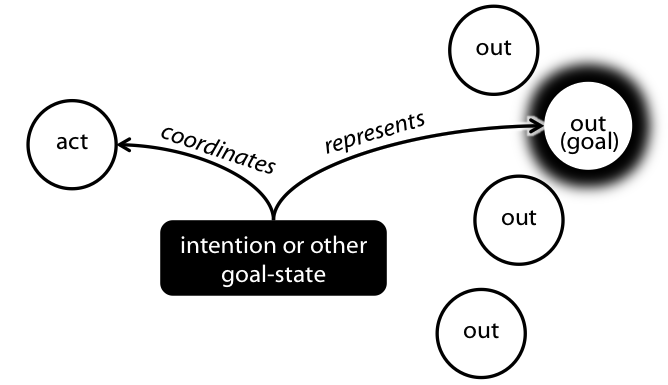
\includegraphics[width=0.3\textwidth]{standard_story.png}
\emph{Figure}: The standard story for individual action.
\end{center}
\end{comment}

\textbf{Distributive goal}.  The \emph{distributive goal} of two or more agents' activities is G: each agent's activities are individually directed to G.

\textbf{Collective goal}.  The \emph{collective goal} of a joint action is G:
(a) each agent’s activities are individually directed to G (i.e. G is a distributive goal);
(b) the agents’ activities are coordinated; and 
(c) coordination of this type would normally  facilitate occurrences of outcomes of G's type




\footnotesize 
\bibliography{$HOME/endnote/phd_biblio}

\end{multicols}

\end{document}